\section{优化步骤}

\subsection{初步优化}

设置完评价函数并确认初始结构满足基本约束后，开始进行自动优化。优化分为三个阶段：

\subsubsection{局部优化（DLS算法）}

首先使用阻尼最小二乘法（Damped Least Squares, DLS）进行局部优化。DLS算法适合在初始解质量较好、像差水平不过于恶劣的情况下使用，收敛速度快\cite{Fischer2008,Zemax2021}。

操作步骤：打开Optimize菜单，选择Local Optimization，算法选择DLS，勾选Auto Update以实时查看2D布局图和像差曲线的变化。观察Merit Function数值，当连续多次迭代后数值趋于稳定（变化量小于0.1\%），停止优化。

初步优化完成后，Merit Function数值相较初始状态下降，点列图弥散斑减小，MTF曲线整体上移，但仍可能存在局部像差（如彗差或场曲）未完全校正的情况。

\begin{figure}[H]
  \centering
  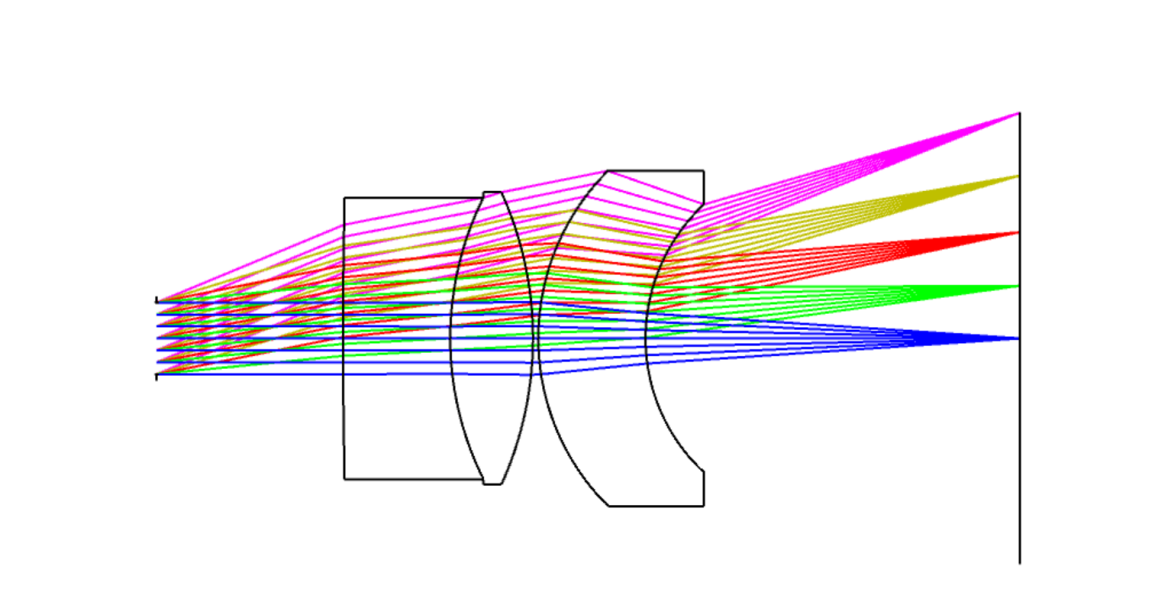
\includegraphics[width=0.95\textwidth]{chapters/chapter4/figures/2D_layout.png}
  \caption{初步优化后2D布局图（Layout）}
  \label{fig:chapter4-layout}
\end{figure}

\begin{figure}[H]
  \centering
  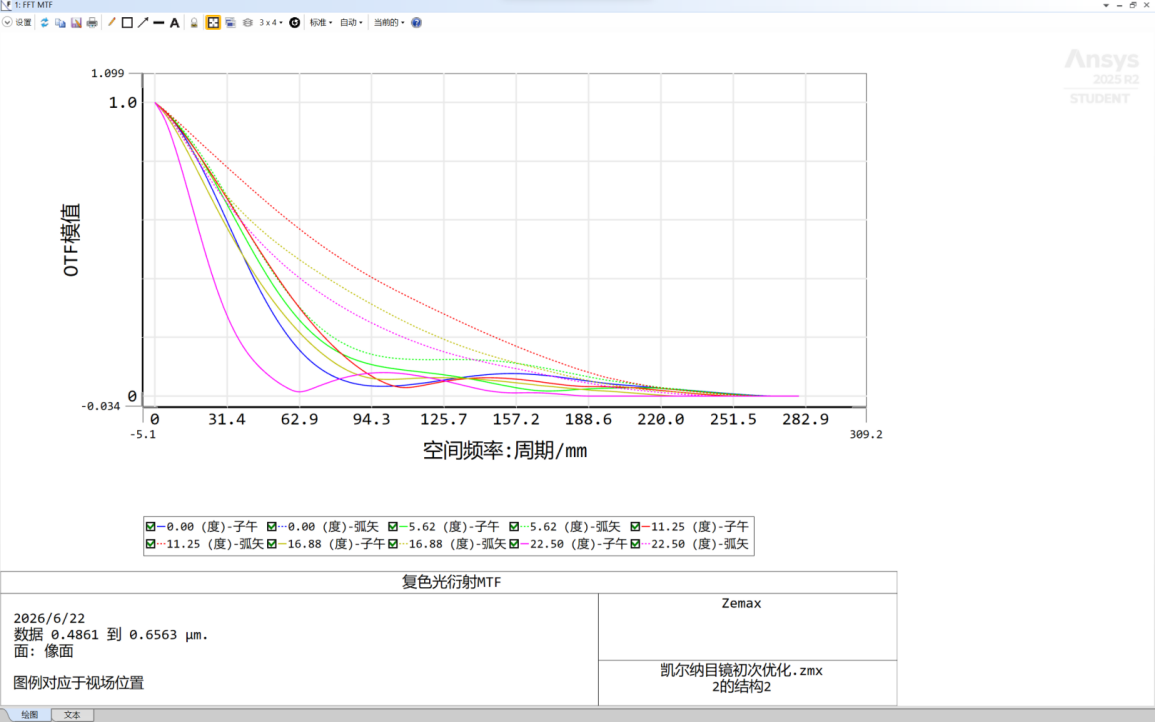
\includegraphics[width=0.95\textwidth]{chapters/chapter4/figures/MTF.png}
  \caption{初步优化后MTF曲线}
  \label{fig:chapter4-mtf}
\end{figure}

\begin{figure}[H]
  \centering
  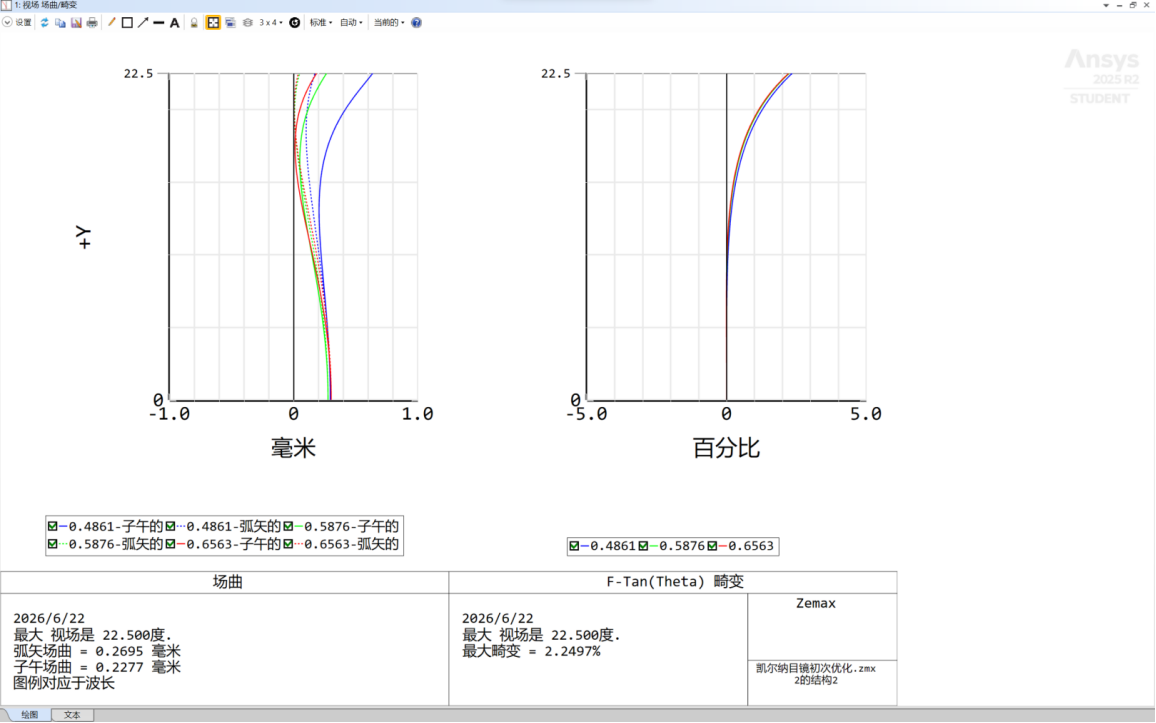
\includegraphics[width=0.95\textwidth]{chapters/chapter4/figures/field_and_distortion.png}
  \caption{初步优化后场曲与畸变图}
  \label{fig:chapter4-field-distortion}
\end{figure}

通过以上分析可以看出，初步优化后的系统在以下方面仍有不足：畸变在全视场边缘仍约为15\%，超过设计指标；全视场相对照度存在一定下降；MTF曲线在高频段仍有较大改善空间。因此，需要进一步进行全局优化和手动调整。

\subsubsection{锤形优化（Hammer Optimization）}

局部优化完成后，运行Hammer Optimization进行全局搜索。锤形优化是Zemax特有的全局优化算法，它在当前局部最优解附近进行大范围扰动，寻找更优的全局解。该方法尤其适用于像差复杂、局部最优解较多的系统。

操作步骤：在Optimize菜单中选择Hammer Optimization，设置运行时间不少于30分钟。优化过程中系统会自动保存当前找到的最优解。锤形优化完成后，从结果列表中选取Merit Function最小且结构合理的方案作为进一步优化的起点。

经过锤形优化后，畸变有所降低，全视场MTF曲线进一步抬升，场曲切向和弧矢焦面的分离度也有所减小。

\subsection{进一步优化思路}

经过初步的局部优化和全局锤形优化后，若部分指标仍未完全达到设计要求，可考虑以下进一步优化策略：

\begin{enumerate}
\def\labelenumi{\arabic{enumi}.}
\item
  调整Merit Function权重：若边缘视场点列半径仍偏大，可提高边缘视场对应TRCX/TRCY操作数的权重，使优化器更关注全视场像质均衡；若系统结构接近厚度边界，则需适当提高MNCA、MNEA、MNCG和MNEG等厚度约束的权重。
\item
  手动微调关键面：根据像差分析结果，对贡献最大像差的面进行手动微调。例如，若彗差主要来自面4（双合镜前表面），可手动调整其曲率半径，然后重新运行DLS优化。
\item
  评价函数升级：当点列图已经满足基本要求时，可在RMS点列半径评价基础上增加波前误差或MTF相关约束，用于进一步控制衍射成像质量。
\item
  玻璃材料替换：若几何形状优化趋于稳定但色差仍偏大，可考虑启用玻璃替换功能，在SCHOTT、CDGM等玻璃库中搜索折射率、阿贝数和可加工性更合适的材料组合。
\item
  分阶段优化：先固定玻璃材料并优化面型、厚度和间隔，待结构稳定后再开放材料或局部结构变量，可降低多变量同时变化导致的收敛不稳定。
\end{enumerate}
